%iffalse
\let\negmedspace\undefined
\let\negthickspace\undefined
\documentclass{article}
\usepackage{cite}
\usepackage{amsmath,amssymb,amsfonts,amsthm}
\usepackage{algorithmic}
\usepackage{graphicx}
\usepackage{textcomp}
\usepackage{xcolor}
\usepackage{txfonts}
\usepackage{listings}
\usepackage{enumitem}
\usepackage{mathtools}
\usepackage{gensymb}
\usepackage{comment}
\usepackage[breaklinks=true]{hyperref}
\usepackage{tkz-euclide} 
\usepackage{listings}
\usepackage{gvv}           
\usepackage{float}
\def\inputGnumericTable{}                                 
\usepackage[latin1]{inputenc}                                
\usepackage{color}                                            
\usepackage{array}                                             
\usepackage{longtable}                                       
\usepackage{calc}                                             
\usepackage{multirow}                                         
\usepackage{hhline}                                           
\usepackage{ifthen}                                           
\usepackage{lscape}
\usepackage{multicol}
\usepackage{amsmath, amssymb}
\usepackage{enumitem}
\usepackage{siunitx}
\usepackage{graphicx}
\usepackage{txfonts}



\newtheorem{theorem}{Theorem}[section]
\newtheorem{problem}{Problem}
\newtheorem{proposition}{Proposition}[section]
\newtheorem{lemma}{Lemma}[section]
\newtheorem{corollary}[theorem]{Corollary}
\newtheorem{example}{Example}[section]
\newtheorem{definition}[problem]{Definition}
\newcommand{\BEQA}{\begin{eqnarray}}
\newcommand{\EEQA}{\end{eqnarray}}
\newcommand{\define}{\stackrel{\triangle}{=}}
\theoremstyle{remark}
\newtheorem{rem}{Remark}
\begin{document}

\bibliographystyle{IEEEtran}
\vspace{3cm}

\title{Clock Project Report}
\author{EE224BTECH11044 - Muthyala koushik% <-this % stops a space
}
\date{}
\maketitle
\bigskip



\renewcommand{\thefigure}{\theenumi}
\renewcommand{\thetable}{\theenumi}



\section{Introduction}
This project implements a digital clock using an AVR microcontroller (e.g., ATmega328P) with a single SN7447 BCD-to-7-segment decoder. The clock displays hours, minutes, and seconds on six multiplexed 7-segment displays. Time is maintained in Binary Coded Decimal (BCD) format and updated every second using a Timer1 compare match interrupt.

\section{Aim}
\begin{itemize}[noitemsep]
    \item Design a digital clock that displays time in \texttt{HH:MM:SS} format.
    \item Use a single SN7447 decoder to drive six 7-segment displays through multiplexing.
    \item Update the time every second via an interrupt-driven timer.
    \item Implement BCD arithmetic to handle digit carry-overs across seconds, minutes, and hours.
\end{itemize}

\section{Components Required}
\begin{itemize}[noitemsep]
    \item AVR Microcontroller (e.g., ATmega328P)
    \item SN7447 BCD-to-7-segment decoder
    \item 6 common anode (or cathode, as required) 7-segment displays
    \item Current-limiting resistors (typically \SI{220}{\ohm} per segment)
    \item External 16\,MHz clock source (or use the internal oscillator if applicable)
    \item Breadboard and connecting wires
\end{itemize}

\section{Hardware Configuration}
\subsection{Pin Connections}
The code defines two groups of connections:
\begin{enumerate}[label=\alph*)]
    \item \textbf{BCD Output to SN7447:}  
    Four AVR pins provide the 4-bit Binary Coded Decimal (BCD) value to the SN7447.
    \begin{center}
    \begin{tabular}{|l|l|l|l|}
    \hline
    \textbf{SN7447 Input} & \textbf{Function} & \textbf{AVR Port/Pin} & \textbf{Digital Pin (Uno)} \\ \hline
    A (LSB) & BCD Data Bit 0 & PD2 & 2 \\ \hline
    B       & BCD Data Bit 1 & PD3 & 3 \\ \hline
    C       & BCD Data Bit 2 & PD4 & 4 \\ \hline
    D (MSB) & BCD Data Bit 3 & PD5 & 5 \\ \hline
    \end{tabular}
    \end{center}

    \item \textbf{Display Multiplex Control:}  
    Six separate AVR pins are used to enable the common pin of each 7-segment display in a multiplexed arrangement.
    \begin{center}
    \begin{tabular}{|l|l|l|l|}
    \hline
    \textbf{Display Digit} & \textbf{Function}       & \textbf{AVR Port/Pin} & \textbf{Digital Pin (Uno)} \\ \hline
    Hours Tens (H1)        & Digit Enable Control   & PD6 & 6 \\ \hline
    Hours Units (H2)       & Digit Enable Control   & PD7 & 7 \\ \hline
    Minutes Tens (M1)      & Digit Enable Control   & PB0 & 8 \\ \hline
    Minutes Units (M2)     & Digit Enable Control   & PB1 & 9 \\ \hline
    Seconds Tens (S1)      & Digit Enable Control   & PB2 & 10 \\ \hline
    Seconds Units (S2)     & Digit Enable Control   & PB3 & 11 \\ \hline
    \end{tabular}
    \end{center}
\end{enumerate}

\subsection{Segment Wiring}
\begin{itemize}[noitemsep]
    \item The outputs of the SN7447 decoder (segments \texttt{a} through \texttt{g}) are connected in parallel to the corresponding segments on all six 7-segment displays.
    \item Each segment connection should include a current-limiting resistor.
    \item The common pins of the displays (anode or cathode, depending on the type) are switched by the multiplex control lines.
\end{itemize}

\subsection{Power Supply}
\begin{center}
\begin{tabular}{|l|l|}
\hline
\textbf{Connection} & \textbf{Notes} \\ \hline
VCC & +5V supply to SN7447, displays, and AVR \\ \hline
GND & Common ground for all components \\ \hline
\end{tabular}
\end{center}

\newpage 

\begin{figure}[h!]
  \centering
  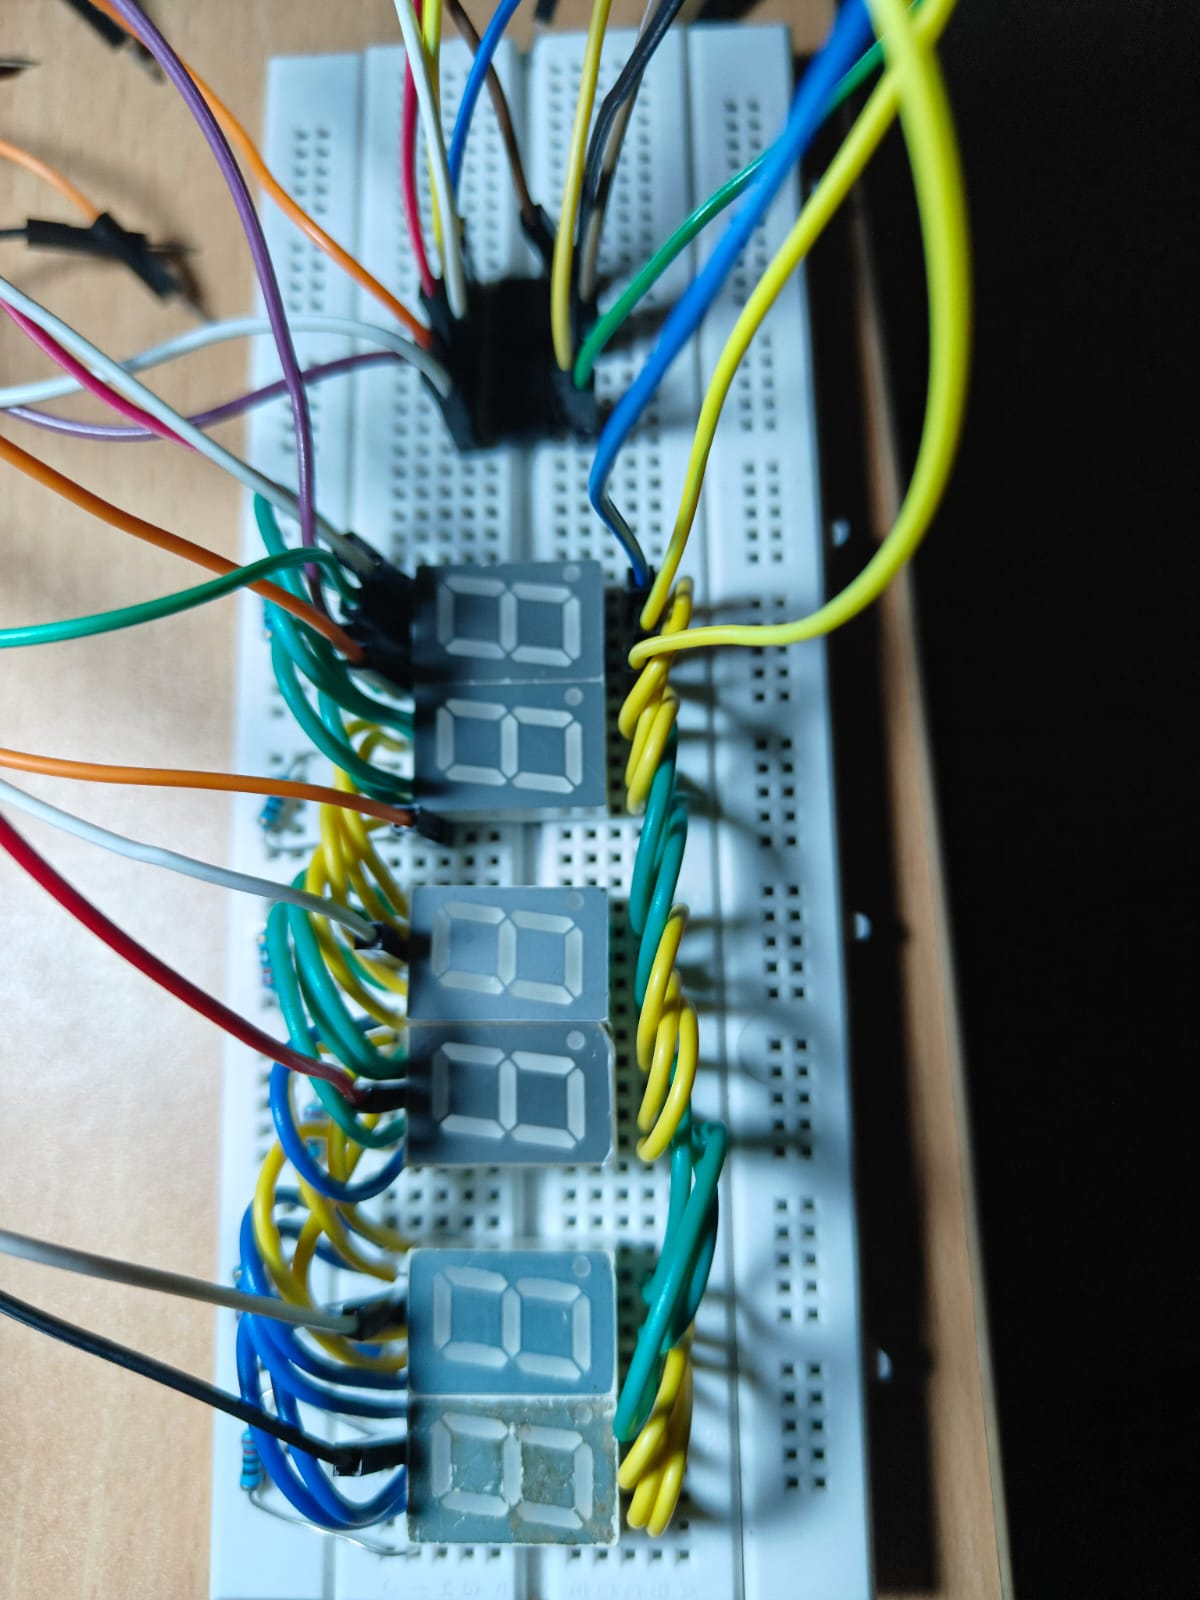
\includegraphics[width=0.7\textwidth]{figs/circuit.png}
  \caption{Block diagram of the digital clock system.}
  \label{fig:clock_diagram}
\end{figure}

\section{Software Design}
\subsection{Overall Architecture}
The project firmware is divided into two main modules:
\begin{enumerate}[label=\alph*)]
    \item \textbf{Time Management:}
    \begin{itemize}[noitemsep]
        \item Time is stored in three volatile BCD variables: \texttt{hours}, \texttt{minutes}, and \texttt{seconds}.
        \item A Timer1 Compare Match interrupt (in CTC mode with a 1024 prescaler) updates the time every second.
        \item BCD arithmetic is used to increment seconds and handle carry-overs for minutes and hours.
    \end{itemize}
    \item \textbf{Display Multiplexing:}
    \begin{itemize}[noitemsep]
        \item The function \texttt{displayTime()} extracts individual digits from the BCD time values.
        \item A single 4-bit BCD digit is sent to the SN7447 via the BCD output pins (PD2--PD5) using the function \texttt{displayDigit()}.
        \item Each digit is displayed in sequence by enabling its corresponding control pin for a brief period (using \texttt{\_delay\_ms()}), creating the illusion of a continuously lit display.
    \end{itemize}
\end{enumerate}

\subsection{Interrupt-Driven Time Update}
\begin{itemize}[noitemsep]
    \item Timer1 is set to CTC mode with a prescaler of 1024, and the compare register is loaded with a value for a 1-second interval.
    \item The ISR (\texttt{TIMER1\_COMPA\_vect}) increments the seconds variable in BCD, performs digit carry operations, and updates minutes and hours accordingly.
\end{itemize}

\section{Operation Workflow}
\begin{enumerate}
    \item \textbf{Initialization:}
    \begin{itemize}[noitemsep]
        \item Configure BCD output pins (PD2--PD5) and display control pins (PD6, PD7, PB0--PB3) as outputs.
        \item Initialize Timer1 and enable global interrupts.
    \end{itemize}
    \item \textbf{Time Update:}
    \begin{itemize}[noitemsep]
        \item Every second, the ISR updates the time variables using BCD arithmetic and carry management.
    \end{itemize}
    \item \textbf{Display Refresh:}
    \begin{itemize}[noitemsep]
        \item The main loop continuously calls \texttt{displayTime()}, which sequentially enables each display digit.
        \item Each digit is shown for a short period, and rapid cycling creates persistence-of-vision.
    \end{itemize}
\end{enumerate}

\section{Performance Specifications}
\begin{itemize}[noitemsep]
    \item \textbf{Voltage:} 5V DC
    \item \textbf{Clock Frequency:} 16\,MHz
    \item \textbf{Time Update Accuracy:} 1-second resolution (via Timer1 interrupt)
    \item \textbf{Multiplexing Rate:} Fast enough to achieve persistence-of-vision across 6 digits
\end{itemize}

\section{Code Explanation}
The following section explains the main parts of the digital clock code implemented on an AVR microcontroller.

\subsection{Preprocessor Directives and Includes}
\begin{itemize}[noitemsep]
    \item \texttt{\#define F\_CPU 16000000UL}: Sets the CPU clock frequency to 16\,MHz. This definition is required by the delay routines from \texttt{<util/delay.h>}.
    \item \texttt{\#include <avr/io.h>}: Includes the definitions for the input/output registers specific to the AVR microcontroller.
    \item \texttt{\#include <avr/interrupt.h>}: Provides the interrupt handling functions and macros.
    \item \texttt{\#include <util/delay.h>}: Enables the use of \texttt{\_delay\_ms()} for creating precise delays.
\end{itemize}

\subsection{Pin Definitions and Hardware Connections}
\begin{itemize}[noitemsep]
    \item \textbf{BCD Pins (for SN7447 Decoder):}  
    \begin{itemize}[noitemsep]
        \item \texttt{A} is defined as \texttt{PD2}
        \item \texttt{B} is defined as \texttt{PD3}
        \item \texttt{C} is defined as \texttt{PD4}
        \item \texttt{D} is defined as \texttt{PD5}
    \end{itemize}
    These pins send the 4-bit BCD value (representing a digit) to the SN7447 decoder.
    
    \item \textbf{Display Control Pins (for Multiplexing):}
    \begin{itemize}[noitemsep]
        \item Hours Tens (H1) is defined as \texttt{PD6}
        \item Hours Units (H2) is defined as \texttt{PD7}
        \item Minutes Tens (M1) is defined as \texttt{PB0}
        \item Minutes Units (M2) is defined as \texttt{PB1}
        \item Seconds Tens (S1) is defined as \texttt{PB2}
        \item Seconds Units (S2) is defined as \texttt{PB3}
    \end{itemize}
    These control pins are used to selectively enable each of the six 7-segment displays via multiplexing.

    \item \textbf{Clock Variables:}  
    The variables \texttt{hours}, \texttt{minutes}, and \texttt{seconds} are declared as volatile \texttt{uint8\_t} and stored in BCD format. For example, \texttt{hours} is initialized to \texttt{0b00010010} (i.e., 12 in BCD).
\end{itemize}

\subsection{Display Functions}
\begin{itemize}[noitemsep]
    \item \texttt{displayDigit(uint8\_t digit)}:  
    This function sends a 4-bit BCD digit to the SN7447 decoder. It modifies \texttt{PORTD} by:
    \begin{itemize}[noitemsep]
        \item Clearing the bits corresponding to PD2--PD5 (using a bit mask).
        \item Shifting the input digit into the correct bit positions.
    \end{itemize}
    
    \item \texttt{displayTime()}:
    \begin{itemize}[noitemsep]
        \item Extracts individual BCD digits for hours, minutes, and seconds.
        \item For each digit (e.g., tens and units of hours, minutes, seconds), the function:
        \begin{enumerate}[noitemsep]
            \item Enables the appropriate display control pin.
            \item Calls \texttt{displayDigit()} to send the digit via the SN7447.
            \item Uses \texttt{\_delay\_ms()} for a brief delay to ensure the digit is visible.
            \item Disables the display control pin before moving to the next digit.
        \end{enumerate}
        \item This rapid cycling through digits (multiplexing) creates the illusion that all six displays are lit continuously.
    \end{itemize}
\end{itemize}

\subsection{Interrupt Service Routine (ISR)}
\begin{itemize}[noitemsep]
    \item \texttt{ISR(TIMER1\_COMPA\_vect)}:  
    This routine is executed once per second, as determined by Timer1.
    \begin{itemize}[noitemsep]
        \item The seconds counter is incremented by one in BCD.
        \item A series of conditional checks manage BCD carry:
        \begin{itemize}[noitemsep]
            \item When the lower nibble exceeds 9, it carries over by adding 0x10 (i.e., 16 in decimal) to the upper nibble.
            \item If the seconds reach 60 (BCD value \texttt{0b01100000}), the seconds reset to 0 and minutes are incremented.
            \item Similar checks apply for minutes and hours, with hours resetting after reaching 24 (BCD value \texttt{0b00100000}).
        \end{itemize}
    \end{itemize}
\end{itemize}

\subsection{Timer Initialization}
\begin{itemize}[noitemsep]
    \item \texttt{timer1\_init()}:
    \begin{itemize}[noitemsep]
        \item Configures Timer1 in CTC (Clear Timer on Compare) mode.
        \item Sets the prescaler to 1024, which divides the 16\,MHz clock.
        \item Loads the Output Compare Register (\texttt{OCR1A}) with the value needed to achieve a 1-second interval.
        \item Enables the Timer1 compare interrupt via \texttt{TIMSK1}.
        \item Calls \texttt{sei()} to globally enable interrupts.
    \end{itemize}
\end{itemize}

\subsection{Main Function}
\begin{itemize}[noitemsep]
    \item \texttt{main()}:
    \begin{itemize}[noitemsep]
        \item Configures the data direction registers:
        \begin{itemize}[noitemsep]
            \item \texttt{DDRD} is set for the BCD output pins (PD2--PD5) and the display control pins for hours (PD6 and PD7).
            \item \texttt{DDRB} is set for the display control pins for minutes and seconds (PB0--PB3).
        \end{itemize}
        \item Calls \texttt{timer1\_init()} to initialize Timer1 and enable interrupts.
        \item Enters an infinite loop in which \texttt{displayTime()} is continuously called. This ensures the display is refreshed rapidly to maintain the appearance of a continuously lit clock.
    \end{itemize}
\end{itemize}
\end{document}
